%%%%%%%%%%%%%%%%%%%%%%%%%%%%%%%%%%%%%%%%%
% Beamer Presentation
% LaTeX Template
% Version 1.0 (10/11/12)
%
% This template has been downloaded from:
% http://www.LaTeXTemplates.com
%
% License:
% CC BY-NC-SA 3.0 (http://creativecommons.org/licenses/by-nc-sa/3.0/)
%
%%%%%%%%%%%%%%%%%%%%%%%%%%%%%%%%%%%%%%%%%

%----------------------------------------------------------------------------------------
%	PACKAGES AND THEMES
%----------------------------------------------------------------------------------------

\documentclass[aspectratio=1610]{beamer}

\mode<presentation> {

% The Beamer class comes with a number of default slide themes
% which change the colors and layouts of slides. Below this is a list
% of all the themes, uncomment each in turn to see what they look like.
\usepackage{amsmath}
\usepackage[russian]{babel}
\usepackage{hyperref}
\usepackage{amssymb}
\usepackage{euscript}
\usepackage{bbold}
\usepackage{amssymb}
\usepackage{mathrsfs}
\usepackage{graphicx}
%\usepackage[usenames]{color}

\DeclareMathOperator{\diag}{diag}
\newtheorem{hypothesis}{Conjecture}
\renewcommand{\proofname}{Доказательство}
\theoremstyle{plain}
\newtheorem{thm}{Теорема} %[section], чтобы нумеровать сначала в каждом разделе
\newtheorem{lm}{Лемма}
\newtheorem{st}{Утверждение}

\theoremstyle{definition}
\newtheorem*{defn}{Определение}
\newtheorem*{ex}{Упр}
\newtheorem*{cor}{Следствие}
\newtheorem*{name}{Обозначение}

\theoremstyle{remark}
\newtheorem*{rem}{Замечание}


\def\geq{\geqslant}
\def\ge{\geqslant}
\def\leq{\leqslant}
\def\le{\leqslant}

\DeclareMathOperator{\supp}{supp}
\DeclareMathOperator{\Id}{Id}
\DeclareMathOperator{\D}{D}

\newcommand{\cuplim}{\bigcup\limits}
\newcommand{\ilim}{\int\limits}
\newcommand{\slim}{\sum\limits}
\newcommand{\maxlim}{\max\limits}
\newcommand{\suplim}{\sup\limits}
\newcommand{\T}{\mathbb{T}}
\newcommand{\dm}{\, d\mu_n}
\newcommand{\R}{\mathbb{R}}
\newcommand{\E}{\mathbb{E}}
\newcommand{\PP}{\mathbb{P}}
\newcommand{\Z}{\mathbb{Z}}
%\newcommand{\R^nn}{\mathbb{R}^n}
%\newcommand{C^1}{\mathbb{C}^1}
\newcommand{\til}{\widetilde}
\newcommand{\dd}{\partial}
\newcommand{\eps}{\varepsilon}

\usetheme{default}
%\usetheme{AnnArbor}
%\usetheme{Antibes}
%\usetheme{Bergen}
%\usetheme{Berkeley}
%\usetheme{Berlin}
%\usetheme{Boadilla}
%\usetheme{CambridgeUS}
%\usetheme{Copenhagen}
%\usetheme{Darmstadt}
%\usetheme{Dresden}
%\usetheme{Frankfurt}
%\usetheme{Goettingen}
%\usetheme{Hannover}
%\usetheme{Ilmenau}
%\usetheme{JuanLesPins}
%\usetheme{Luebeck}
%\usetheme{Madrid}
%\usetheme{Malmoe}
%\usetheme{Marburg}
%\usetheme{Montpellier}
%\usetheme{PaloAlto}
%\usetheme{Pittsburgh}
%\usetheme{Rochester}
%\usetheme{Singapore}
%\usetheme{Szeged}
%\usetheme{Warsaw}

% As well as themes, the Beamer class has a number of color themes
% for any slide theme. Uncomment each of these in turn to see how it
% changes the colors of your current slide theme.

%\usecolortheme{albatross}
%\usecolortheme{beaver}
%\usecolortheme{beetle}
%\usecolortheme{crane}
%\usecolortheme{dolphin}
%\usecolortheme{dove}
%\usecolortheme{fly}
%\usecolortheme{lily}
%\usecolortheme{orchid}
%\usecolortheme{rose}
%\usecolortheme{seagull}
%\usecolortheme{seahorse}
%\usecolortheme{whale}
%\usecolortheme{wolverine}

%\setbeamertemplate{footline} % To remove the footer line in all slides uncomment this line
\setbeamertemplate{footline}[page number] % To replace the footer line in all slides with a simple slide count uncomment this line

\setbeamertemplate{navigation symbols}{} % To remove the navigation symbols from the bottom of all slides uncomment this line
}
\DeclareMathOperator{\Vol}{Vol}
\usepackage{graphicx} % Allows including images
\usepackage{booktabs} % Allows the use of \toprule, \midrule and \bottomrule in tables
%\usepackage {tikz}
\usepackage{tkz-graph}
\GraphInit[vstyle = Shade]
\tikzset{
  LabelStyle/.style = { rectangle, rounded corners, draw,
                        minimum width = 2em, fill = yellow!50,
                        text = red, font = \bfseries },
  VertexStyle/.append style = { inner sep=5pt,
                                font = \normalsize\bfseries},
  EdgeStyle/.append style = {->, bend left} }
\usetikzlibrary {positioning}
%\usepackage {xcolor}
\definecolor {processblue}{cmyk}{0.96,0,0,0}
%----------------------------------------------------------------------------------------
%	TITLE PAGE
%----------------------------------------------------------------------------------------

\title[Short title]{Кодирование случайных множеств в булевой модели с переменной интенсивностью} % The short title appears at the bottom of every slide, the full title is only on the title page

\author{Давыденкова Мария Сергеевна\\\medskip
Научный руководитель: Лифшиц Михаил Анатольевич \\
Рецензент: Белопольская Яна Исаевна} 
\institute[SPBU] 
{
Санкт-Петербургский государственный университет
\medskip
}
\date{18 июня 2020\,г.} % Date, can be changed to a custom date

\begin{document}

\begin{frame}
\titlepage % Print the title page as the first slide
\end{frame}

\begin{frame}{Средняя ошибка дискретизации}
Пусть $S$  ---  случайный элемент некоторого метрического пространства $(X, dist)$.

\begin{defn}
Средней ошибкой дискретизации $S$ называется величина  $$D^{(q)}(r) := \inf\limits_{\#\mathcal{C}\leq e^r}\E \min\limits_{A\in\mathcal{C}}dist(S, A), \quad r>0.$$
\end{defn}{}

Важной характеристикой распределения $S$ является оценка скорости убывания этой величины при стремлении $r$ к бесконечности.

\end{frame}

\begin{frame}{Булева модель}

В данной задаче в качестве случайного элемента пространства компактов с метрикой Хаусдорфа выступает {\it Булева модель случайного множества}.
\medskip

Рассмотрим куб $[0,a]^d$ в $\R^d$ и  случайный набор шаров: 
\begin{itemize}
    \item центры шаров $\xi_i \sim \mathcal{U}[0, a]^d$;
    \item радиусы $R_i \geq 0$ одинаково распределены;
    \item  количество шаров $N\sim\mathcal{P}(a^d\lambda)$, где $\lambda = \lambda(a)$.
\end{itemize}   
Все эти случайные величины независимы. 

\begin{defn}
Булева модель случайного множества:
$$S_a = \cuplim_{i=1}^N B(\xi_i, R_i) \cap [0,a]^d.$$
\end{defn}


    
\end{frame}

\begin{frame}{Минимальное число видимых шаров $K_a$}
\begin{center}
  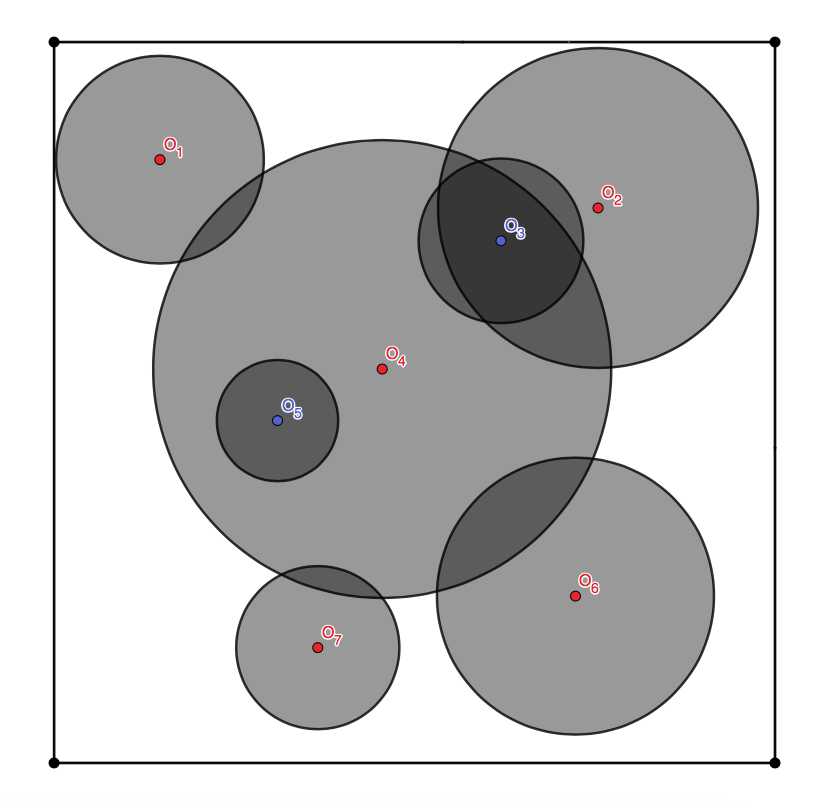
\includegraphics[scale = 0.5]{pic1.png}  
\end{center}

%\begin{multline*}
%    K_a = \min \{r \geq 1 | \exists i_1, \ldots , i_r \subset \{1, \ldots , N\} :\\ S_a = \cuplim_{l=1}^r B(\xi_{i_l}, R_{i_l}) \cap [0,a]^d
%    \}.
%\end{multline*}


%Вероятности больших уклонений этой величины играют важную роль в оценке скорости убывания средней ошибки дискретизации.

\end{frame}{}

\begin{frame}{Вероятности больших уклонений $K_a$} 
Будем предполагать, что $n\gg a^d\lambda$.

\begin{itemize}
    \item Тривиальная оценка:
$$ \PP[K_a \geq n] \leq 
    \exp(-n\log n + dn\log a + n\log\lambda + 
    O(n)), \ n, a\to \infty.$$
    
    \item {\it Ф.~Аурзада, М.~Лифшиц (2019, J. Complexity)} изучали случай $a=1,\ \lambda = const$ и показали, что для некоторых распределений $R_i$ выполнено 
$$\PP[K_1 \geq n] = \exp(-\beta\cdot n\log n\cdot (1 + o(1))), \quad n\to\infty.$$
Константа $\beta > 1$ зависит от размерности $d$, нормы в $\R^d$ и распределения радиусов.
\end{itemize}

\end{frame}

%\begin{frame}{Полученные результаты: одномерный случай}%

%Отдельно рассматривается случай $d=1$.
%\begin{thm}
%Пусть $n\gg a\lambda, n\gg a$. Тогда
%\begin{itemize}
%    \item если распределение $R_1$ имеет плотность $p(z)\approx z^{\alpha-1}$ для $z\to 0$ и некоторого $\alpha > 0$:
%\end{itemize}
%    \begin{multline*}
%    \PP[K_a\geq n] = \exp(-(1+\alpha)n\log n + (1+\alpha)n\log a
%    +n\log\lambda +O(n)), \\n,a \to\infty.
%\end{multline*}\begin{itemize}
%\item если $R_1\equiv r>0$ п.н.:
%\begin{equation*}
%    \PP[K_a\geq n] = 0
%\end{equation*}
%для достаточно больших  $n$ и $a$.
%\end{itemize}
%\end{thm}
    
%\end{frame}



\begin{frame}{Полученные результаты}
Рассмотрим случай $d \geq 2$.
\begin{thm}
Пусть $n\gg a^d\lambda, n\gg a^d$. Тогда
\begin{itemize}
    \item если распределение $R_1$ имеет плотность $p(z)\approx z^{\alpha-1}$ для $z\to 0$ и некоторого $\alpha > 0$:
    \begin{equation*}
    \PP[K_a\geq n] = \exp(-\textcolor{red}{(1+\alpha/d)}\cdot n\log n + \textcolor{red}{(1+\alpha/d)} \cdot dn\log a 
    +n\log\lambda +O(n)),\quad 
    n,a \to\infty.
\end{equation*}
\item если $R_1\equiv r>0$ п.н.:
\begin{equation*}
    \PP[K_a\geq n] = \exp(-\textcolor{red}{\beta} \cdot n\log n + \textcolor{red}{\beta}\cdot dn\log a 
    +n\log\lambda +O(n)),\quad 
    n,a \to\infty.
\end{equation*}

\end{itemize}
\end{thm}


\end{frame}{}

\begin{frame}{Два подхода к решению задачи}

{\it Первый подход:} для некоторых распределений были найдены события $E_1$ и $E_2$:
$$\PP[E_1] \leq \PP[K_a \geq n] \leq \PP[E_2].$$
{\it Пример:}
\begin{center}
 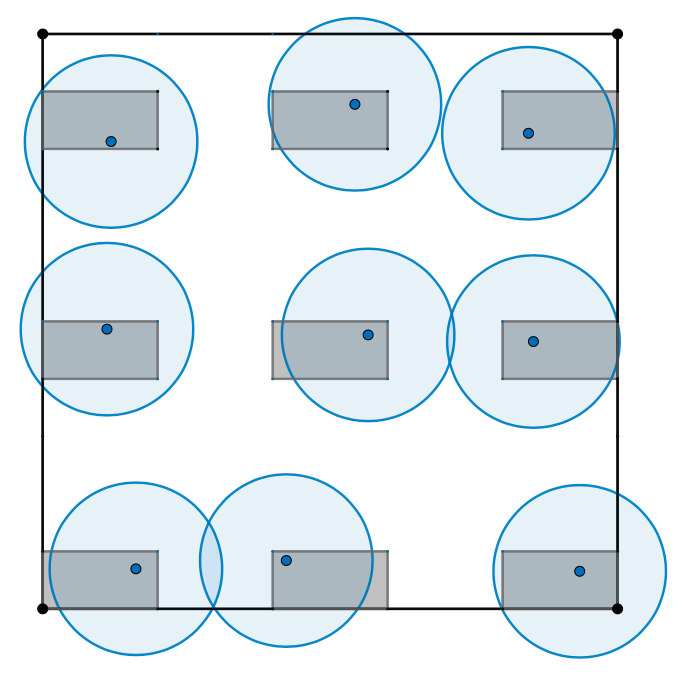
\includegraphics[scale = 0.3]{pic2.png}   
\end{center}



\end{frame}
\begin{frame}{Два подхода к решению задачи}

{\it Второй подход:} сведение к задаче для куба постоянного размера. Были доказаны теоремы, позволяющие получить из оценок для случая $a=1$ оценки для параметра $a$, стремящегося к бесконечности.
    
\end{frame}

\begin{frame}{Сведение к задаче для куба постоянного размера}

\begin{thm}[Нижняя оценка]
    Пусть $R_1\leq r$ п.н. для некоторого $r>0$, $d\geq 1$, $n \gg a^d\lambda$, и $n\gg a^d$. 
Предположим, что 
\begin{equation*}
    \PP[K_1 \geq n] \geq \exp \left(-\beta\cdot n\log n + \gamma\cdot n\log\lambda + O(n)\right),\  n \to \infty.
 \end{equation*}{}
Тогда 
\begin{equation*}
    \PP[K_a \geq n] \geq \exp \left(-\beta\cdot n\log n + \textcolor{red}{\beta\cdot dn\log a} + \gamma\cdot n\log\lambda + O(n)\right),\quad  n, a \to \infty.
\end{equation*}{}
\end{thm}
    
\end{frame}

\begin{frame}{Сведение к задаче для куба постоянного размера}

\begin{thm}[Верхняя оценка]
    Пусть $d\geq 1$,  $n \gg a^d\lambda$ и $n \gg a^d$. Обозначим через $K_a^{(b)}$ минимальное число видимых шаров в картинке с радиусами, увеличенными в $b$ раз.
Предположим, что для любого числа $b \in (0, 1)$ верно следующее:
\begin{equation*}
    \PP[K_1^{(b)} \geq n] =\PP[K_1 \geq n] \leq \exp \left(-\beta\cdot n\log n + \gamma\cdot n\log\lambda + O(n)\right),\quad  n \to \infty.
\end{equation*}
    


Тогда 
\begin{equation*}
    \PP[K_a \geq n] \leq \exp \left(-\beta\cdot n\log n + \textcolor{red}{\beta\cdot dn\log a} + \gamma\cdot n\log\lambda + O(n)\right),\quad  n, a \to \infty.
\end{equation*}{}
\end{thm}
    
\end{frame}

\begin{frame}{Поведение $K_a$ при малых $\lambda$}

Отдельно изучался случай, когда $n\gg a^d\lambda$, но неверно, что $n\gg a^d$. Было доказано следующее утверждение.

\begin{thm}
    Пусть $\lambda = \lambda(a)$ таково, что $a^d\lambda^2 \to 0$ при $a\to\infty$, и случайная величина $R_1$ имеет $d$-й момент, $d\geq 1$. Тогда $$\PP[K_a < N] \to 0, \  a\to\infty.$$
\end{thm}

То есть для достаточно быстро убывающих $\lambda$ выполнено $K_a \sim N$ при $a\to\infty$.
    
\end{frame}


\begin{frame}
\begin{center}
\Huge Спасибо за внимание.
\end{center}
\end{frame}

\end{document}
